% IEEE SPMB conference paper (Paper track). Target length: 6 pages.
% Compile: pdflatex paper && bibtex paper && pdflatex paper && pdflatex paper
% Requires IEEEtran.cls (https://www.ctan.org/pkg/ieeetran) and references.bib.
% Figures are under experiments/results/ (PNG, 300 DPI). The figure* environments (Figs. 1
% and 4) are double-column and are the first knobs for fitting exactly 6 pages.
\documentclass[conference]{IEEEtran}
\usepackage{graphicx}
\usepackage{amsmath}
\usepackage{booktabs}
\usepackage{cite}
\usepackage{url}
\graphicspath{{experiments/results/}}

\begin{document}

\title{Correctness Criteria for Windowed Real-Time EEG Signal Processing:\\
Phase, Windowing, and Spectral Estimation}

\author{\IEEEauthorblockN{Sukalyan Roy}
\IEEEauthorblockA{Avinya Neurotech\\
Email: sukalyanroy2003@gmail.com}}

\maketitle

\begin{abstract}
Browser- and cloud-based clinical EEG review increasingly filters and re-references signals on
demand, one short window at a time, rather than on whole recordings. We show that this windowed,
real-time setting introduces correctness failures that whole-signal offline practice does not
anticipate, and we derive deterministic criteria that prevent them. Using a standard-library
reference implementation evaluated against synthetic ground truth and multiple open clinical
recordings (PhysioNet CHB-MIT), we establish three results. First, filtering display windows
independently produces chunk-seam artifacts; an overlap-add scheme that filters an extended
window and keeps the clean center removes them by about 35\,dB on synthetic data and more on real
EEG, at negligible latency. Second, zero-phase forward--backward filtering (\texttt{filtfilt})
has a length floor of three filter lengths; a window shorter than the floor cannot be filtered
zero-phase, so a streaming filter must fall back to a causal path whose uncompensated group delay
displaces events by up to about 500\,ms---a clinically meaningful, regime-dependent error. We
show the floor and the shift scale as $3(\mathrm{order}+1)$ and $(\mathrm{taps}-1)/2/f_s$ across
FIR orders, distill the design rule $\mathrm{chunk}+2\!\cdot\!\mathrm{overlap}\ge 3\!\cdot\!
\mathrm{taps}$, and confirm both on multiple CHB-MIT subjects. Third, in windowed spectral
estimation, tapering the analysis window before an estimator that already tapers biases relative
band power by up to about 12 percentage points for Welch and 9 for multitaper; tapering once
removes it. The contribution is a small, reproducible set of correctness invariants for streaming
clinical EEG signal processing.
\end{abstract}

\begin{IEEEkeywords}
EEG, real-time filtering, zero-phase filtering, overlap-add, group delay, quantitative EEG,
spectral estimation, reproducibility.
\end{IEEEkeywords}

\section{Introduction}
Clinical electroencephalography (EEG) is increasingly reviewed through networked, on-demand
viewers that fetch and process short windows of a recording rather than loading entire studies.
This shift moves standard digital-signal-processing (DSP) operations---bandpass and notch
filtering and quantitative-EEG (QEEG) feature extraction---from a whole-signal, offline setting
into a windowed, real-time setting. Operations that are textbook-correct offline can become
subtly and silently wrong under windowing: a filter that is zero-phase on a whole recording may
not be on a short window, and an estimator that is unbiased on a clean buffer may be biased once
a window is tapered upstream.

This paper characterizes that gap and derives deterministic criteria to close it. Rather than
propose a new algorithm, we take the standard streaming DSP chain---an FIR bandpass applied with
\texttt{scipy.signal.filtfilt}, an IIR notch, and a Welch/multitaper power spectral density
(PSD) routine---as the system under test, and quantify where windowing breaks correctness. We use
synthetic signals with known spectra for ground truth and open clinical recordings for external
validity. We make four contributions:
\begin{enumerate}
\item A reproducible methodology that turns a windowed DSP chain into a correctness benchmark,
built only on standard libraries, with released code and data fetched at run time.
\item A zero-phase length-floor result: below a length threshold \texttt{filtfilt} cannot run, so
a streaming filter falls back to a causal path, producing a measured event mis-timing of up to
$\sim$500\,ms; we give a deterministic guard and generalize it across FIR order.
\item A quantification of overlap-add windowed filtering ($\sim$35\,dB seam-artifact reduction at
negligible latency), confirmed on multiple real CHB-MIT subjects.
\item A cascaded-tapering result for windowed PSD estimation: tapering twice biases relative band
power for both Welch and multitaper, with a one-line remedy.
\end{enumerate}

\section{Background and Related Work}
\textbf{Streaming and real-time EEG visualization.} Networked EEG viewers serve windowed segments
to the client; the European Data Format (EDF/EDF+) is the de-facto storage
format~\cite{kemp1992,kemp2003}. Prior work emphasizes interactivity and scale; the DSP
correctness of windowed filtering and feature extraction in this setting is largely unexamined.

\textbf{EEG filtering and phase.} Bandpass and notch filtering are standard, and the risks of
phase distortion and filter transients on event timing are documented for offline
analysis~\cite{widmann2015,decheveigne2019}. Zero-phase (forward--backward) filtering removes
phase distortion but is non-causal and requires sufficient data length~\cite{oppenheim2009}.
These works warn about phase offline; none characterize the length-gated transition from a
zero-phase to a causal regime inside a streaming filter, or its effect on event timing.

\textbf{Block convolution and boundary artifacts.} Filtering long signals in blocks is classically
handled by overlap-add/overlap-save~\cite{oppenheim2009,proakis2007}, with routines provided by
standard libraries~\cite{virtanen2020}. The textbook methods are not characterized for clinical
EEG streaming, nor parameterized against a zero-phase length floor.

\textbf{Spectral band power and QEEG.} Relative band power via Welch~\cite{welch1967} or
multitaper~\cite{thomson1982} estimation is a common QEEG feature, with reference implementations
in wide use~\cite{gramfort2013,virtanen2020}. Tapering is intrinsic to these estimators;
implementation-level errors that taper a second time, and their bias on clinical relative band
power, are under-reported.

\section{Methods}
\subsection{Reference DSP primitives}
We evaluate the conventional streaming chain implemented with standard libraries only: an FIR
bandpass (order 200, 202 taps, designed with \texttt{firwin} and a Hamming window) applied with
forward--backward zero-phase filtering (\texttt{scipy.signal.filtfilt}); an IIR notch
(\texttt{iirnotch}) applied with \texttt{filtfilt}; and a Welch/multitaper PSD routine
(\texttt{scipy.signal.welch}, \texttt{mne}). A salient and standard detail is that
\texttt{filtfilt} requires the input to exceed its default padding length,
$3\!\cdot\!\mathrm{len(taps)}$ samples; a streaming filter that must return a shorter window
therefore has to use a causal filter (\texttt{lfilter}) instead. The reference implementation
(\texttt{dsp.py}) makes both regimes explicit.

\subsection{Synthetic ground truth}
We generate deterministic, seeded multichannel signals at 200\,Hz with known spectral content:
band-limited oscillations ($\delta/\theta/\alpha/\beta$) with randomized phases,
amplitude-modulated bursts, $1/f$ background, and a 50\,Hz mains component. The signal is
continuous and stationary-in-expectation, so any discontinuity in a windowed reconstruction is
attributable to the windowing strategy rather than to the signal.

\subsection{Windowing strategies and metrics}
We compare three strategies driving the \emph{same} filters: \emph{whole-signal} (zero-phase
reference), \emph{naive} per-window (each non-overlapping window filtered independently), and
\emph{overlap-add} (each window filtered within an extended window of $\pm$\,overlap seconds of
real neighbors, retaining the center). \emph{Boundary error} is the RMS error within $\pm$50\,ms
of seams versus the reference; \emph{interior error} excludes $\pm$0.6\,s. \emph{Event
mis-timing} is the shift of a 20\,ms Gaussian transient by peak location and cross-correlation.
For spectral estimation, \emph{feature equivalence} compares per-band relative power from the
estimator under test to \texttt{mne} (\texttt{psd\_array\_welch}/\texttt{psd\_array\_multitaper})
by Pearson correlation and maximum per-band discrepancy in percentage points (pp).

\subsection{Real data and reproducibility}
We confirm the filtering results on PhysioNet CHB-MIT~\cite{shoeb2009,goldberger2000} (256\,Hz,
bipolar montage), using the first recording of each of \textbf{10} subjects. Experiments ran
in a fixed environment (Python 3.12; NumPy 2.4.1; SciPy 1.17.0; MNE 1.11.0). The reference
implementation, synthetic generators, metrics, and figure scripts are released; raw EDFs are
fetched from PhysioNet at run time and are not redistributed.

\begin{figure*}[t]
\centering
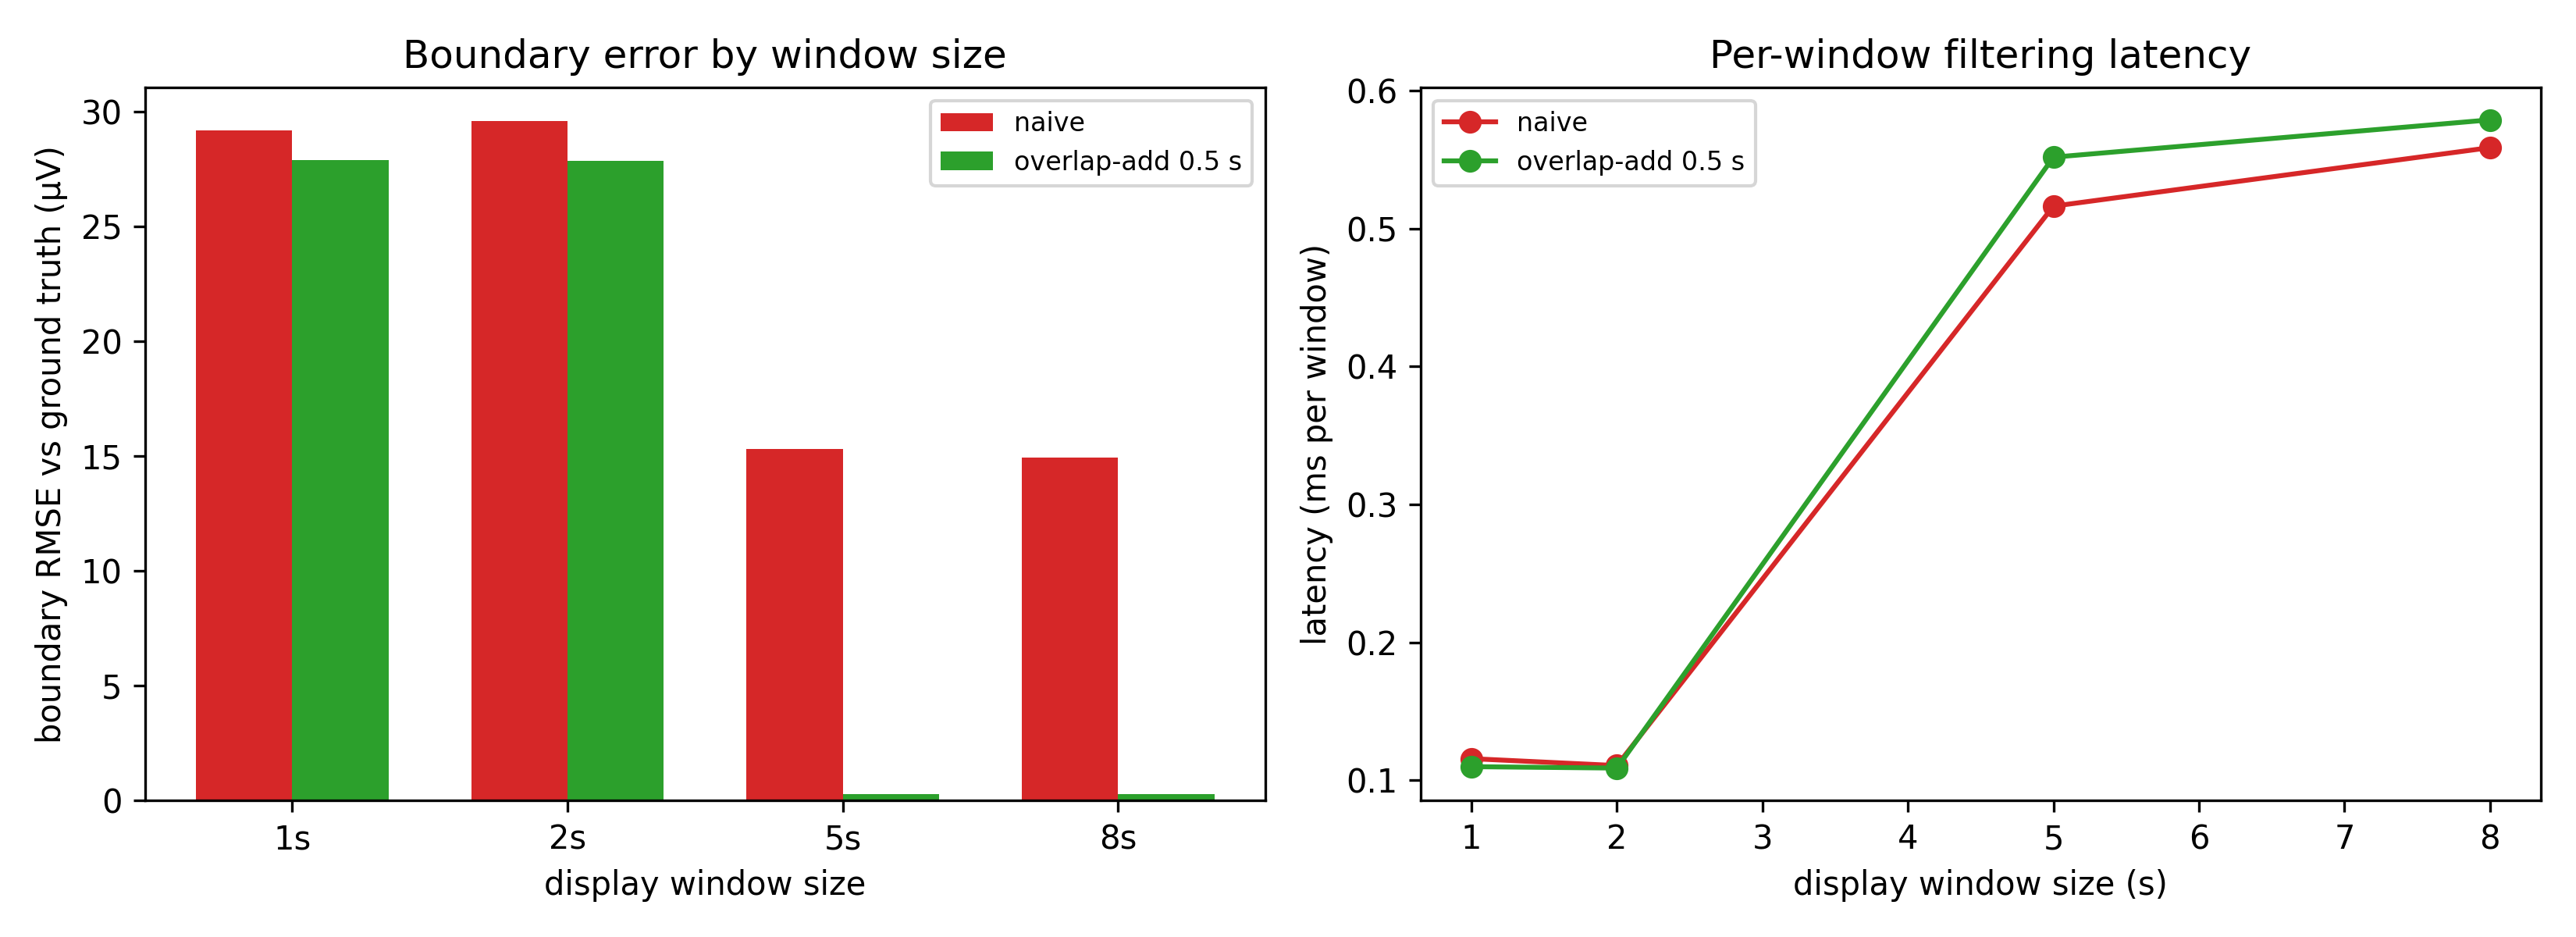
\includegraphics[width=0.78\textwidth]{fig_summary.png}
\caption{Boundary RMSE by display-window size (left) and per-window filtering latency (right):
overlap-add removes the seam error across window sizes at near-identical latency.}
\label{fig:summary}
\end{figure*}

\section{Results}
\subsection{R1: Overlap-add eliminates window-seam artifacts}
With 8\,s windows, naive filtering concentrates error at seams (boundary RMSE 14.93\,$\mu$V) while
leaving the interior near-exact; overlap-add with 0.5\,s context reduces boundary RMSE to
0.275\,$\mu$V (34.7\,dB), and 1.0\,s renders it negligible (Figs.~\ref{fig:seam}--\ref{fig:summary}).
The per-window overhead is within a few percent of naive filtering, so the correction is
effectively free.

\begin{figure}[t]
\centering
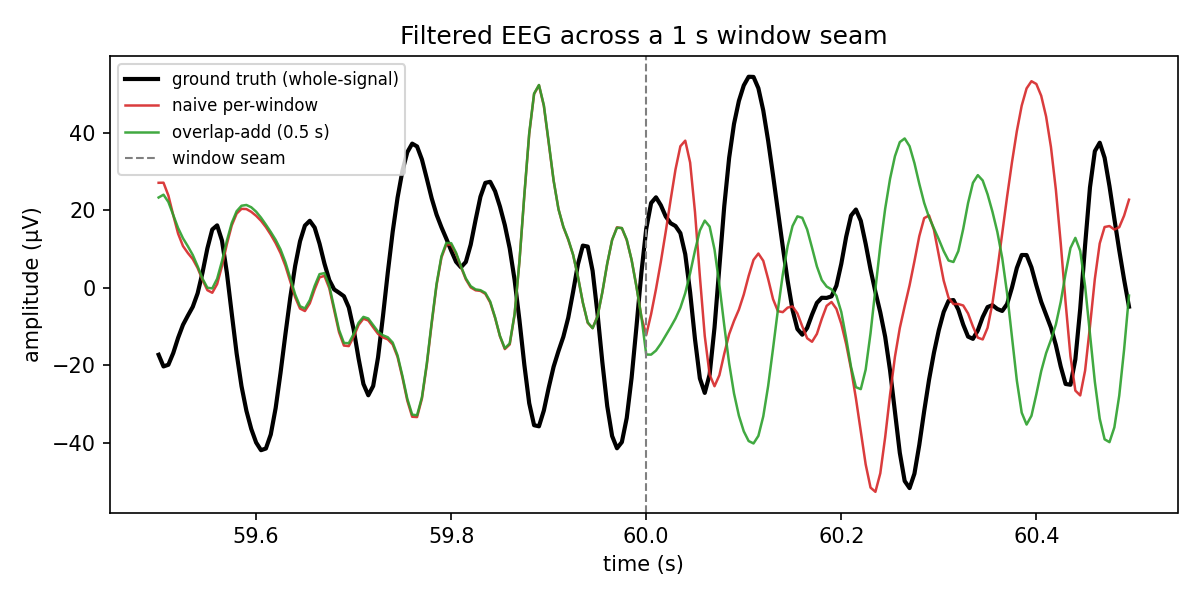
\includegraphics[width=\columnwidth]{fig_seam.png}
\caption{Filtered synthetic EEG across a 1\,s window seam. Naive per-window filtering departs from
the whole-signal ground truth at the seam; overlap-add (0.5\,s context) tracks it.}
\label{fig:seam}
\end{figure}

\subsection{R2: A zero-phase length floor and a design criterion}
The bandpass is zero-phase via \texttt{filtfilt} only when the window exceeds
$3\!\cdot\!\mathrm{taps} = 606$ samples (3.03\,s at 200\,Hz); a shorter window cannot be filtered
zero-phase. A streaming filter processes a span of $\mathrm{chunk}+2\!\cdot\!\mathrm{overlap}$:
large windows clear the floor and are zero-phase, but a small window (e.g.\ a 1\,s chunk with
0.5\,s overlap spans $400 < 606$ samples) falls below it. On the causal fallback the error is
large \emph{throughout} the window (interior RMSE 30.7\,$\mu$V), not only at seams. The
deterministic guard is to keep
\begin{equation}
(\mathrm{chunk}+2\!\cdot\!\mathrm{overlap})\,f_s \;\ge\; 3\!\cdot\!\mathrm{len(taps)},
\label{eq:criterion}
\end{equation}
i.e.\ at least 1.01\,s of overlap each side for a 1\,s chunk at 200\,Hz.

\subsection{R3: Magnitude fidelity and event mis-timing}
On the zero-phase path the magnitude response realizes the design: interior passband (1--25\,Hz)
gain $-0.64\pm1.54$\,dB, with the 50\,Hz notch and 60\,Hz stopband below the $-120$\,dB
measurement floor (Fig.~\ref{fig:mag}). The timing is regime-dependent: a 20\,ms transient is
unshifted (0\,ms) on the zero-phase path but is displaced by $+500$\,ms on the causal fallback,
equal to the uncompensated linear-phase FIR group delay
$(\mathrm{taps}-1)/2/f_s\approx502$\,ms (Fig.~\ref{fig:shift}). Combined with R2, whenever a
window is short enough to force the fallback, displayed events---central to spike review and
annotation alignment---are mis-timed by about half a second.

\begin{figure}[t]
\centering
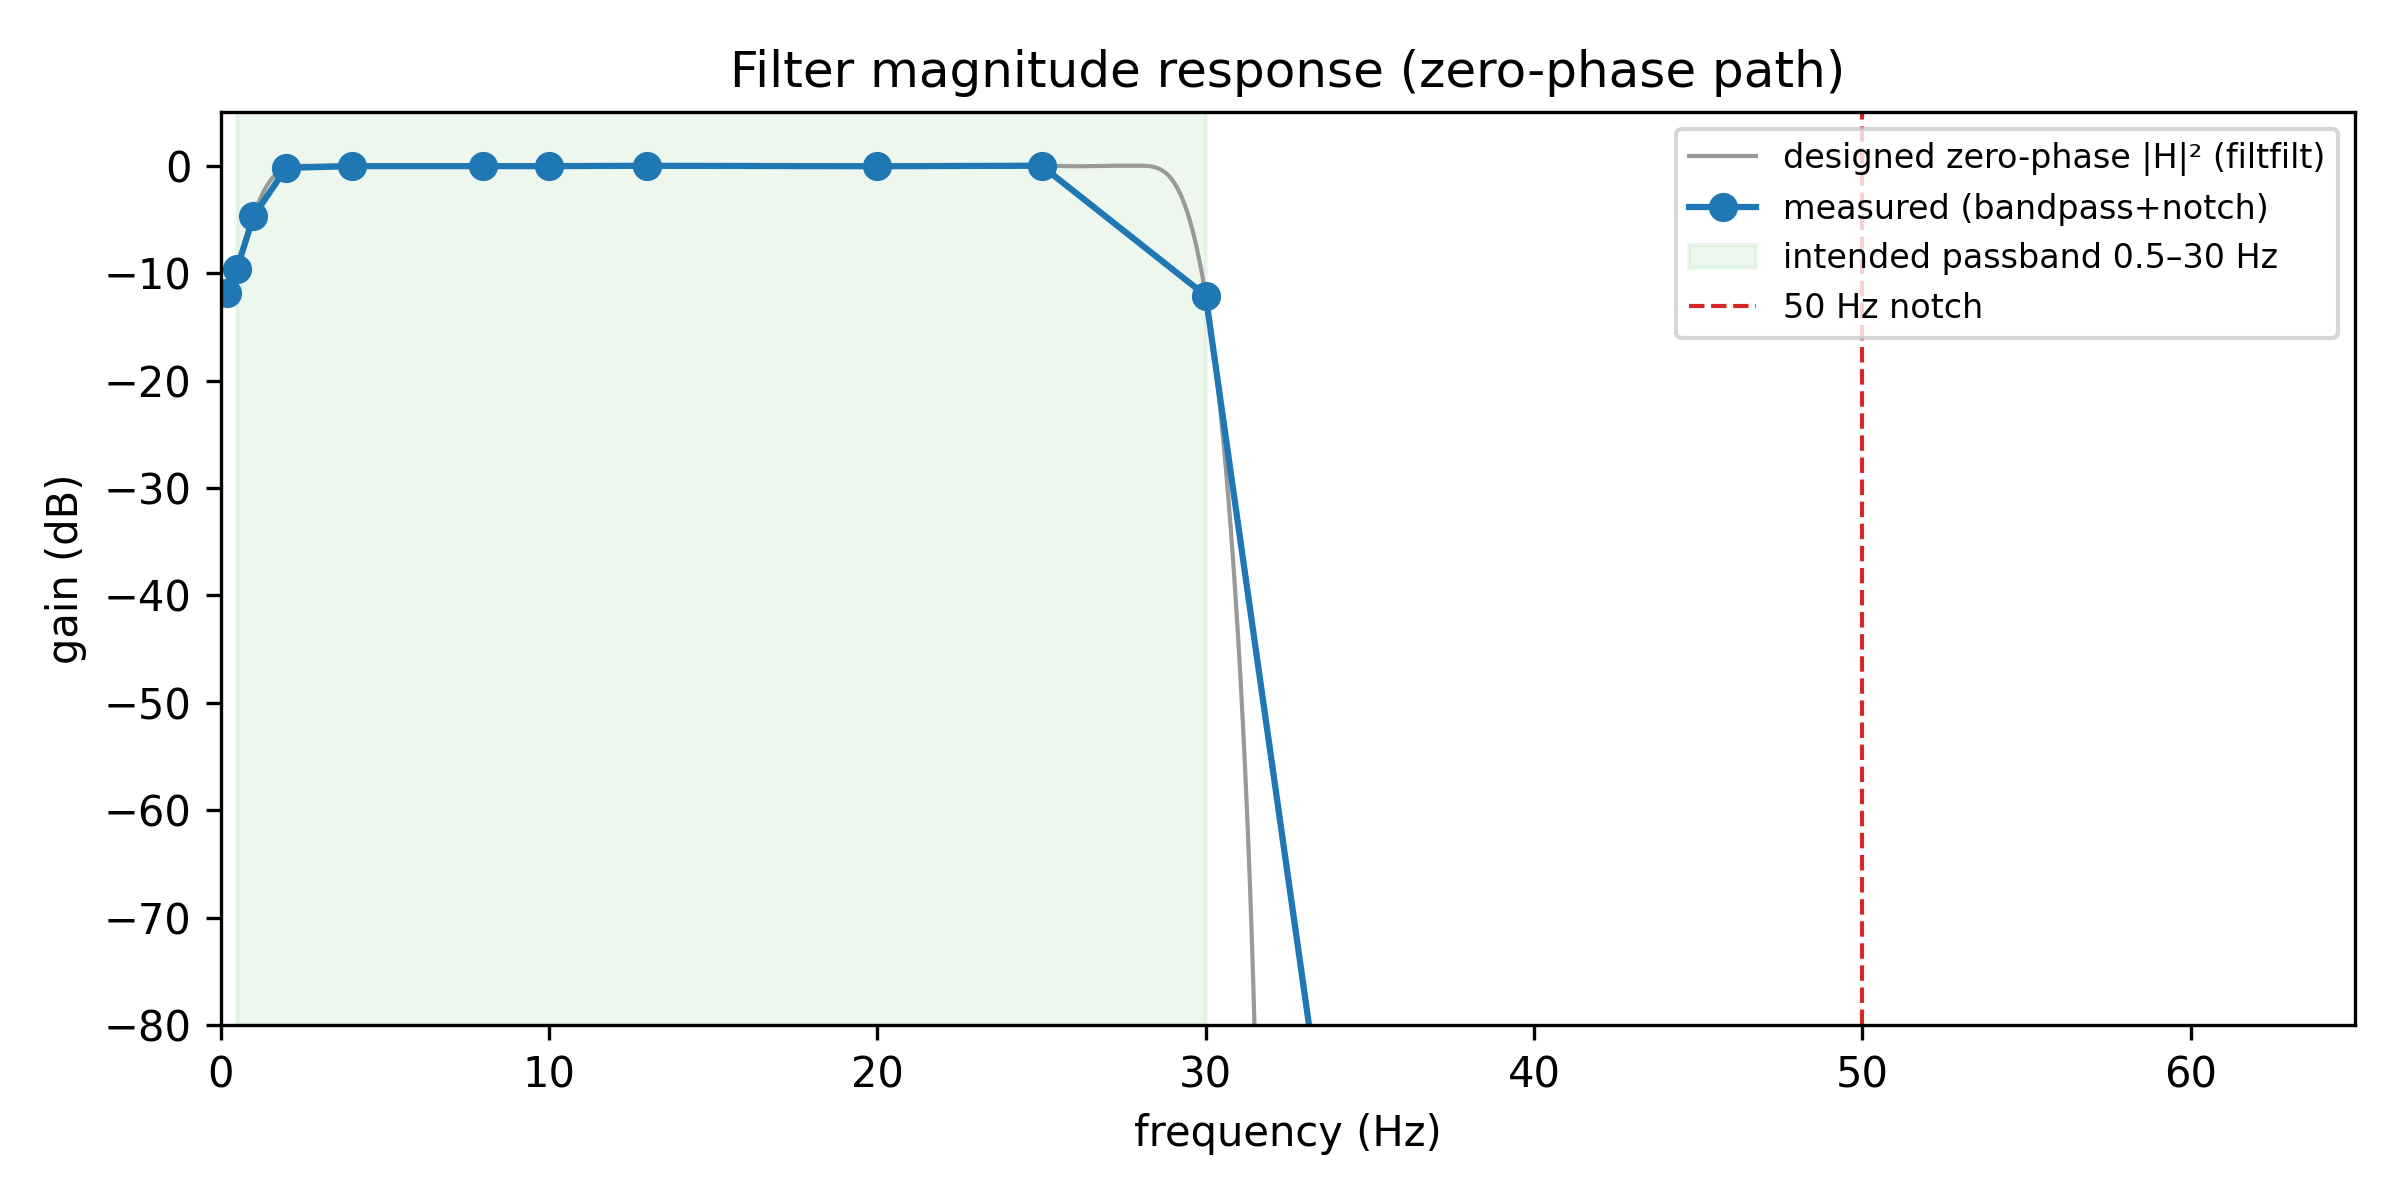
\includegraphics[width=\columnwidth]{fig_magnitude.png}
\caption{Filter magnitude response (zero-phase path): the intended 0.5--30\,Hz passband and the
50\,Hz notch are realized; measured gains match the designed $|H|^2$.}
\label{fig:mag}
\end{figure}

\begin{figure}[t]
\centering
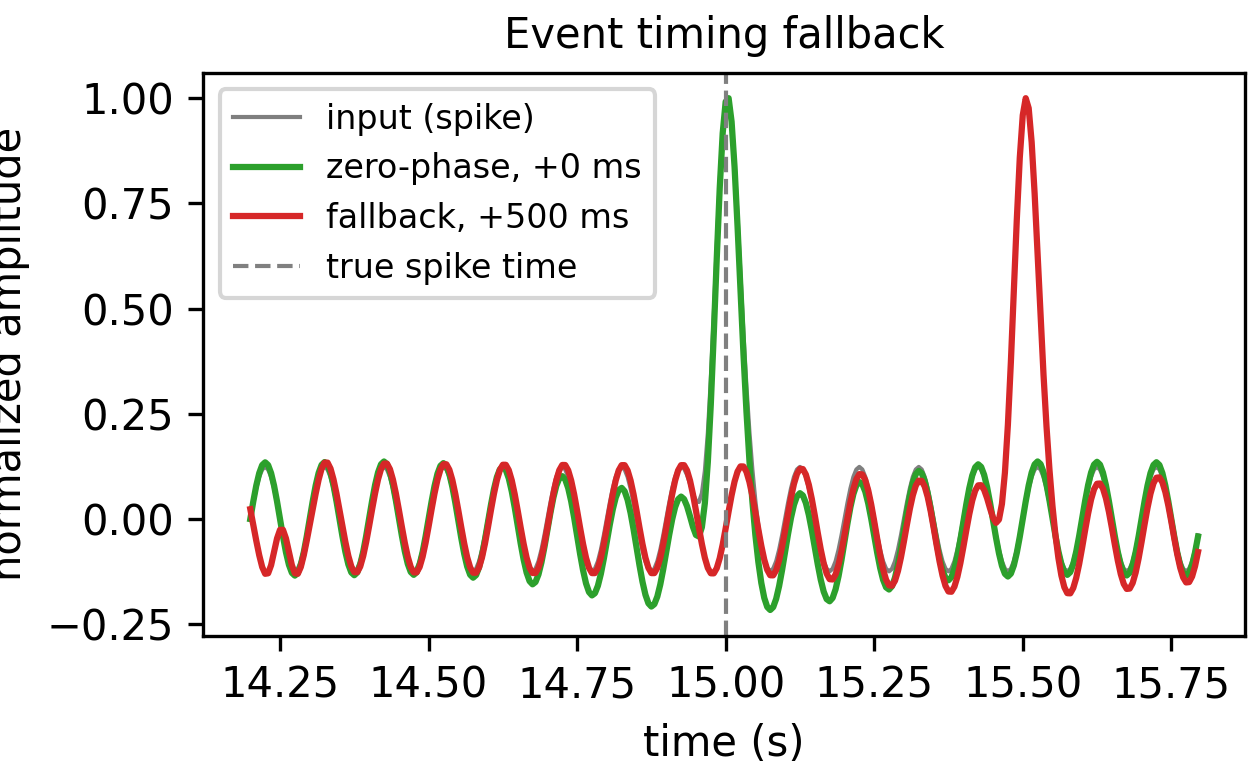
\includegraphics[width=\columnwidth]{fig_transient_shift.png}
\caption{Event timing for a 20\,ms transient: the zero-phase path preserves timing (0\,ms); the
short-window causal fallback shifts the event by $+500$\,ms.}
\label{fig:shift}
\end{figure}

\subsection{R4: Generalization across FIR order and robustness}
The floor equals $3(\mathrm{order}+1)$ taps and the fallback shift equals
$(\mathrm{taps}-1)/2/f_s$; both scale with FIR order (Table~\ref{tab:order}, Fig.~\ref{fig:order}).
Sweeping the total filtered length through the floor shows boundary error collapse sharply at the
threshold (Fig.~\ref{fig:transition}). Across 12 seeds the overlap-add reduction is
$35.1\pm2.3$\,dB (naive $15.9\pm4.1\,\mu$V; overlap-add $0.273\pm0.035\,\mu$V), confirming
robustness and generalizing criterion~\eqref{eq:criterion} to any FIR order.

\begin{table}[t]
\caption{Zero-phase floor and fallback shift scale with FIR order (200\,Hz).}
\label{tab:order}
\centering
\begin{tabular}{cccc}
\toprule
FIR order & taps & floor (samples / s) & fallback shift (ms) \\
\midrule
100 & 102 & 306 / 1.53 & 255 \\
200 & 202 & 606 / 3.03 & 505 \\
300 & 302 & 906 / 4.53 & 755 \\
400 & 402 & 1206 / 6.03 & 1005 \\
\bottomrule
\end{tabular}
\end{table}

\begin{figure}[t]
\centering
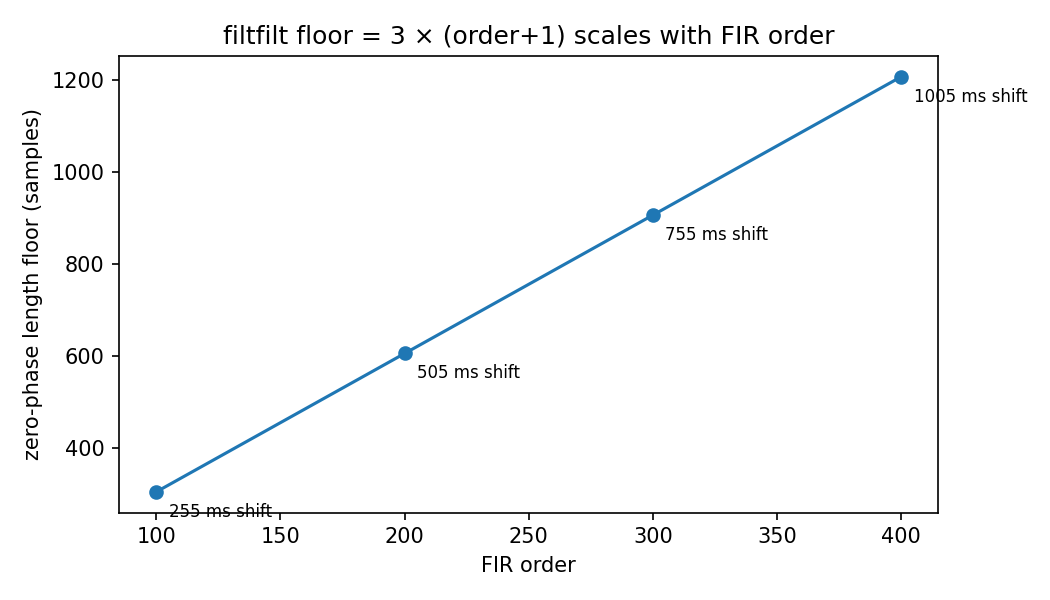
\includegraphics[width=\columnwidth]{fig_order_floor.png}
\caption{The zero-phase length floor $3(\mathrm{order}+1)$ and the annotated fallback group-delay
shift both scale with FIR order.}
\label{fig:order}
\end{figure}

\begin{figure}[t]
\centering
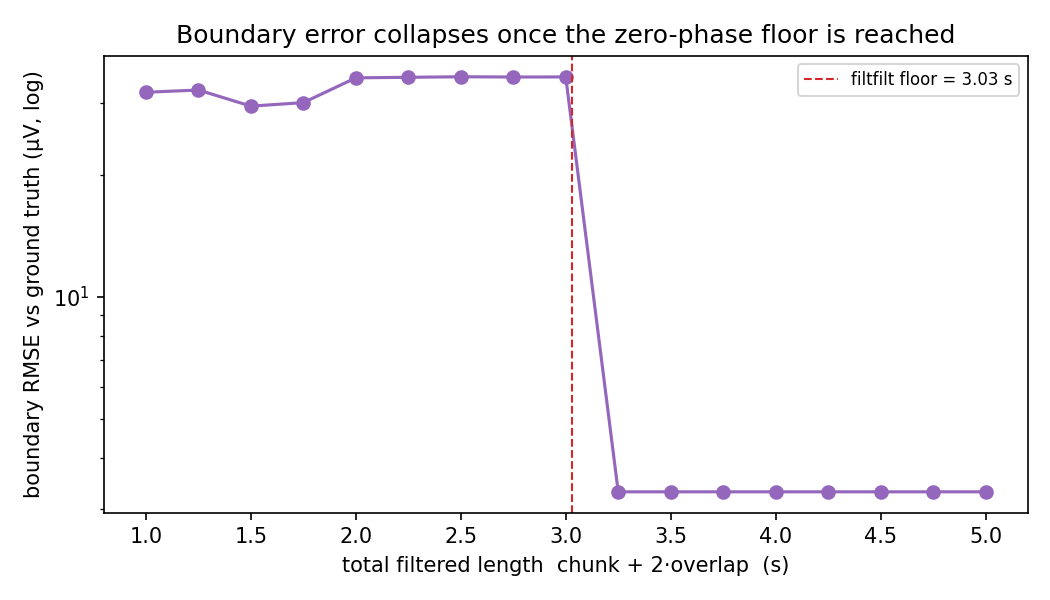
\includegraphics[width=\columnwidth]{fig_transition.png}
\caption{Boundary RMSE versus total filtered length $\mathrm{chunk}+2\!\cdot\!\mathrm{overlap}$:
the error collapses once the length crosses the zero-phase floor.}
\label{fig:transition}
\end{figure}

\subsection{R5: A cascaded-tapering pitfall in spectral estimation}
Welch and multitaper estimators taper internally. Applying a Hann window to the analysis window
\emph{before} such an estimator tapers the signal twice and biases relative band power. A
doubly-tapered Welch estimate differs from MNE \texttt{psd\_array\_welch} by up to 11.9\,pp on the
dominant band; tapering once (letting Welch apply its per-segment Hann) matches MNE to 0.64\,pp
($r=0.99997$, Table~\ref{tab:bp}). The bias is estimator-agnostic: pre-windowing before a
multitaper estimator biases relative band power by up to 9.1\,pp, and removing it recovers the
plain multitaper reference. The remedy is to taper exactly once.

\begin{table}[t]
\caption{Relative band power: max per-band discrepancy vs.\ a single-taper reference of the same
estimator family (8 trials).}
\label{tab:bp}
\centering
\begin{tabular}{lc}
\toprule
Estimator / tapering & max discrepancy (pp) \\
\midrule
Welch, double taper (manual Hann + welch)   & 11.9 \\
Welch, single taper (welch only)            & 0.64 \\
Multitaper, pre-Hann then DPSS tapers       & 9.1  \\
Multitaper, DPSS tapers only                & 0.0  \\
\bottomrule
\end{tabular}
\end{table}

\subsection{R6: Multi-subject real-data confirmation (CHB-MIT)}
On the first recording of \textbf{10} CHB-MIT subjects (256\,Hz), overlap-add reduces seam
boundary RMSE by \textbf{$50.6\pm2.2$}\,dB---comparable to or larger than synthetic---with near-zero
interior error confirming zero-phase behavior (Fig.~\ref{fig:real}). The floor is 606 samples,
i.e.\ 2.37\,s at 256\,Hz; because it is fixed in samples its duration scales with $f_s$. The
fallback shift, measured by cross-correlation against the zero-phase output, is
\textbf{$389\pm7$}\,ms, matching the predicted $(\mathrm{taps}-1)/2/f_s$
(|measured$-$theory| $=$ \textbf{$4.0\pm6.5$}\,ms); the mis-timing is thus sampling-rate-dependent
($\sim$393\,ms at 256\,Hz vs.\ $\sim$500\,ms at 200\,Hz). Per-subject values are consistent
(Table~\ref{tab:ms}): the overlap-add reduction is 47--55\,dB across subjects and the fallback
shift clusters tightly around the predicted group delay.

\begin{figure}[t]
\centering
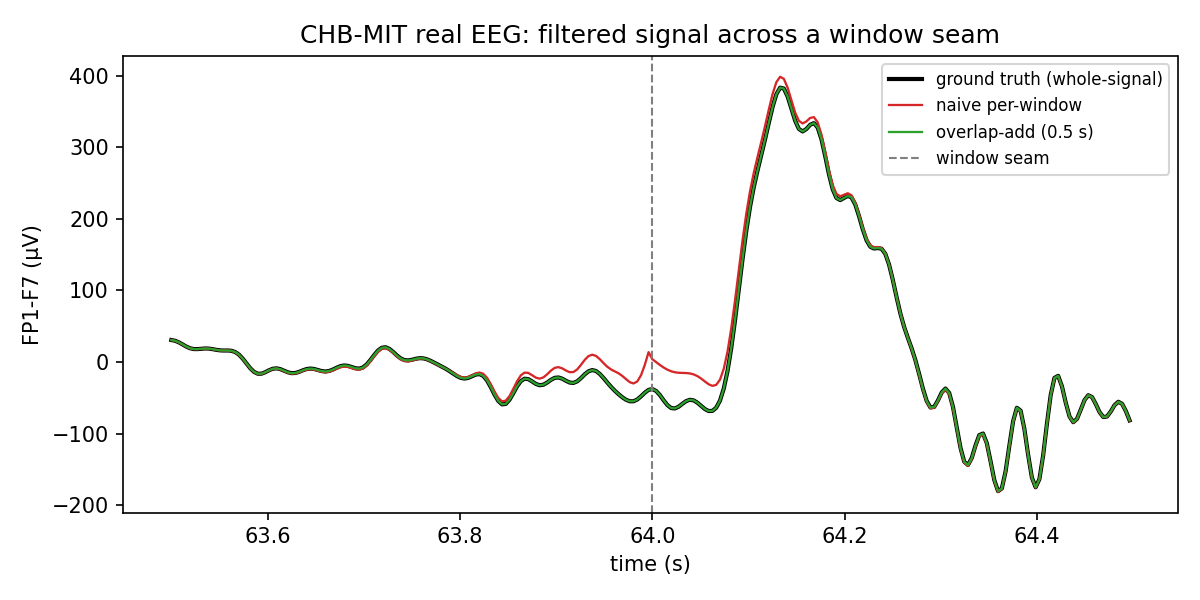
\includegraphics[width=\columnwidth]{fig_realdata_seam.png}
\caption{CHB-MIT real EEG across a window seam: naive filtering deviates at the seam; overlap-add
matches the whole-signal reference.}
\label{fig:real}
\end{figure}

\begin{table}[t]
\caption{Per-subject CHB-MIT confirmation (first recording, 256\,Hz, 8\,s windows). Predicted
group delay $(\mathrm{taps}-1)/2/f_s = 393$\,ms.}
\label{tab:ms}
\centering
\begin{tabular}{lcc}
\toprule
Subject & overlap-add reduction (dB) & fallback shift (ms) \\
\midrule
chb01 & 48.5 & 391 \\
chb02 & 48.7 & 391 \\
chb03 & 52.6 & 369 \\
chb04 & 55.0 & 393 \\
chb05 & 51.1 & 391 \\
chb06 & 47.4 & 391 \\
chb07 & 51.2 & 391 \\
chb09 & 48.7 & 391 \\
chb10 & 52.3 & 391 \\
chb11 & 50.1 & 391 \\
\midrule
mean\,$\pm$\,SD & $50.6\pm2.2$ & $389\pm7$ \\
\bottomrule
\end{tabular}
\end{table}

\section{Discussion}
The results reduce to a small set of correctness invariants for streaming clinical EEG DSP.
(1)~\emph{Windowing:} always supply real context and retain only the center (overlap-add).
(2)~\emph{Zero-phase length:} enforce criterion~\eqref{eq:criterion} so the filter never leaves
the zero-phase regime, and make any fallback observable; otherwise event timing can be off by
hundreds of milliseconds. (3)~\emph{Spectral estimation:} taper exactly once. These are
implementation invariants, not new algorithms, yet each is violated by a plausible windowed
configuration, and each violation is silent in the sense that the output looks like a valid
signal or spectrum.

\emph{Threats to validity.} R1--R4 rest on deterministic properties of the implementation (the
\texttt{filtfilt} length floor; linear-phase FIR group delay) and hold independent of signal
content; we nonetheless confirm them on multiple real recordings (R6). R5 follows from the
algebra of cascaded tapering and is reproduced for two estimator families. We evaluate one
reference implementation, but the invariants follow from properties of \texttt{filtfilt},
linear-phase FIR group delay, and Welch/multitaper tapering common to widely used libraries, and
are relevant to medical-device software life-cycle assurance~\cite{iec62304}.

\section{Conclusion}
Moving routine EEG DSP into a windowed, real-time setting introduces silent correctness failures
that offline practice does not anticipate. By evaluating a standard-library reference chain
against synthetic ground truth and multiple open clinical recordings, we identify and quantify
three---seam artifacts, a zero-phase length-floor fallback with $\sim$500\,ms event mis-timing,
and a cascaded-tapering spectral bias---and give deterministic, low-cost remedies expressible as
short invariants. Future work extends the confirmation to larger cohorts and to montage and
feature-level correctness.

\section*{Reproducibility}
The reference implementation, synthetic generators, metrics, and figure scripts are released; raw
clinical EDFs are downloaded from PhysioNet at run time. All reported numbers are produced by the
released scripts in a pinned environment.

\bibliographystyle{IEEEtran}
\bibliography{references}

\end{document}
